\usetikzlibrary{arrows.meta}
\usepackage{tikz-cd}
\begin{document}
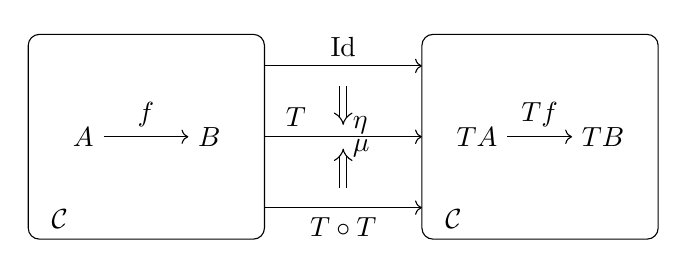
\begin{tikzpicture}
  \draw[rounded corners] (-1.5,-1.3) rectangle (1.5,1.3);
  \draw[rounded corners] (3.5,-1.3) rectangle (6.5,1.3);
  \node at (-1.1,-1.05) {$\mathcal{C}$};
  \node at (3.9,-1.05) {$\mathcal{C}$};
  \node (A) at (-0.8,0) {$A$};
  \node (B) at (0.8,0) {$B$};
  \node (TA) at (4.2,0) {$TA$};
  \node (TB) at (5.8,0) {$TB$};
  \draw[->] (A) -- node[above] {$f$} (B);
  \draw[->] (TA) -- node[above] {$Tf$} (TB);
  \draw[->] (1.5,0.9) -- node[above] {$\mathrm{Id}$} (3.5,0.9);
  \draw[->] (1.5,0) -- node[above, pos=0.2] {$T$} (3.5,0);
  \draw[->] (1.5,-0.9) -- node[below] {$T\circ T$} (3.5,-0.9);
  \draw[double, double distance=2pt, -{Implies[length=6pt]}] (2.5,0.65) -- (2.5,0.15) node[right] {$\eta$};
  \draw[double, double distance=2pt, -{Implies[length=6pt]}] (2.5,-0.65) -- (2.5,-0.15) node[right] {$\mu$};
\end{tikzpicture}
\end{document}
